\chapter{基于秘密分享和随机排列的高效隐私保护机器学习}
基于密码学隐私保护机器学习框架面临着非线性激活函数开销大的问题,而拆分学习和其他混合方法往往面临着中间结果产生的隐私泄漏问题。
%
为此,本文混合秘密分享技术和随机排列技术,使用秘密分享协议计算矩阵乘法等线性运算,同时基于随机排列进行逐元素的非线性激活函数计算,提出了高效易用的隐私保护神经网络框架。
%
本文也对随机排列后的中间结果的隐私泄露程度进行了量化分析,表明随机排列可以有效地保护数据隐私。
%


\label{chap:ss-perm}
\section{研究背景}
随着机器学习在各个领域的广泛应用,数据隐私问题日益严重。
%
训练机器学习模型所需的数据可能分散在多个参与方中,比如两家医院分别有患者的CT图像数据和患者的心电图数据;银行和电商平台分别有用户的金融数据和消费数据。
%
直接把数据汇聚到一个服务器上进行中心化的模型训练,会直接暴露参与方的数据隐私。
%
类似地,在机器学习模型的部署应用阶段,用户需要将数据发送给服务器来获得模型的预测结果,这也暴露了用户的隐私数据。

%
为了解决隐私问题,许多隐私保护机器学习的方案被提出。
%
比如(横向)联邦学习(Federated Learning)~\cite{yangqiang2019federated,mcmahan_2017_fedavg}通过各方训练本地模型再聚合的方式,保护各方本地数据不出域。
但是其仅支持数据横向分割(各个参与方有不同的训练样本,但是样本的特征列是相同的)的情况,且在联邦学习过程中,模型的参数信息也会被暴露给各个参与方。
%
此外,联邦学习主要针对模型训练场景,无法在模型推断阶段提供隐私保护。
%
对于更加复杂的数据纵向分割(各个参与方有同样的样本,但是特征列不同)的情况,或是用户使用模型对自身的输入进行推断的情形,传统的横向联邦学习就无法被应用。
%
拆分学习技术~\cite{vepakomma2018split}可以适用于数据纵向分割或是模型推断的场景。
但是由于在拆分学习的训练和推断过程中,各方需要交换中间结果,因此存在较大的隐私泄漏风险,带来了诸多安全性质疑~\cite{abuadbba2020can_split,hezecheng_2019_model_inversion_attack}。
尽管第\ref{chap:randomized_topk}、\ref{chap:peloss}章提出的方案一定程度上缓解了拆分学习的隐私泄露问题,但是拆分学习交换中间结果的特性注定其无法做到对数据或模型隐私的完全保护,因此在某些安全性要求较高的领域难以应用。

为了实现计算过程中完全的、可证明的隐私保护,必须采用密码学的安全计算技术。
%
近年来,许多基于密码学的隐私保护机器学习框架被提出~\cite{mohassel2017secureml,wagh2019securenn,mohassel2018aby3}。
%
这些框架一般假设有2方或3方参与隐私保护的机器学习计算,采用秘密分享、同态加密、混淆电路等密码学基础技术,来实现安全的神经网络的推断和训练。
%
尽管基于密码学的隐私保护机器学习框架拥有可证明的安全性,其也存在着严重的效率问题。
相比于中心化的明文计算,密码学方法的通信和计算开销往往高出几个数量级。
%
由于使用密码学方法进行算术运算(加法、乘法)的技术已经相对成熟,密码学方法的性能瓶颈往往在于神经网络中的激活函数。
%
神经网络中的激活函数是非线性的,其无法用算术运算简单表示,因此需要使用开销相对较高的混淆电路协议~\cite{yao1986gc}、GMW协议~\cite{gmw_1987}或是其他的定制化协议进行安全计算,并以分段线性~\cite{mohassel2017secureml}或多项式~\cite{gilad2016cryptonets}等方法对非线性函数进行拟合。
%
另一方面,近年来也有一些研究通过将密码学与其他方法结合,设计更加高效的隐私保护机器学习框架~\cite{zhangqiao_2018_gelu_net,xiepeichen_2019_bayhenn,zhou_2022_codesign}。
%
但是这些研究一般采用了类似拆分学习的思想,部分暴露了中间结果的信息,因此存在一定程度的数据或模型的隐私泄露~\cite{wong_2020_lwe_model,abuadbba2020can_split,hezecheng_2019_model_inversion_attack}。
%
因此,如何更好地将密码学方法与非密码学方法结合以提高效率,同时尽可能地保持安全性,成为了隐私保护机器学习中亟待解决的问题。

\section{问题描述}
本节我们先探究暴露模型中间结果带来的隐私泄露问题,然后定义本章所解决的三方协作的隐私保护机器学习问题。

\subsection{隐层表征的隐私泄露}
在拆分学习或部分密码学和拆分学习等其他方法混合的隐私保护机器学习框架中,模型的部分隐层表征会暴露~\cite{zhangqiao_2018_gelu_net,vepakomma2018split,fu2022blindfl,zhou_2022_codesign}。
%
这些研究对于安全性的论证往往基于中间表征的不可逆性质,也就是在没有辅助信息的情况下,从拆分表征恢复出原始的输入特征是不可能的。
%
比如考虑全连接神经网络的第一层表征$\bvec h=W \bvec x$,其中$W \in \mathbb R^{d_1 \times d_0}$是第一层的权重(这里忽略偏置项),$X \in \mathbb R^{d_0}$表示输入表征。
%
即使攻击者收集到了大量隐层表征$H = (\bvec h_1, \cdots, h_n)$,只需要隐层表征维度$d_1$小于输入特征维度$d_0$,线性方程组
\begin{equation}
\begin{cases}
    \bvec h_1 = W \bvec x_1 \\
    \cdots \\
    \bvec h_n = W \bvec x_n \\
\end{cases}
\end{equation}
就是有无穷多解的。
%
这是因为其已知量的个数 $nd_1$ 小于未知量的个数 $d_0d_1 + nd_0$。
%
尽管一些研究在特定条件下提出了对隐层表征进行攻击从而恢复训练特征的办法,但是这些方法往往需要一些额外信息,比如底部模型权重$W$,或是部分泄露的样本-表征对$(\bvec x_i, \bvec h_i)$。
%
接下来我们将说明,即使攻击者只搜集隐层表征,而没有模型的额外信息,依然存在隐私泄露的问题。

\textbf{样本间距离信息的隐私泄露}:
%
Johnson-Lindenstrauss引理~\cite{matouvsek_2008_jl_lemma}告诉我们,对高维数据点的低维线性投影可以很大程度上保留数据点之间的距离关系。
%
也就是说,
\begin{equation}
    \Vert W \bvec x_1 - W \bvec x_2 \Vert \approx c\Vert \bvec x_1 - \bvec x_2 \Vert,    
\end{equation}
其中$c$是一个和$W$的分布以及维度相关的常数。
%
考虑到神经网络的全连接层也可以视为一个随机线性投影,因此隐层表征之间的距离也可以反应原始输入特征之间的距离,从而使得整个数据集的拓扑结构信息被暴露。
%
以MNIST数据集~\cite{mnist}为例,我们将784维的输入图片通过一个按照正态分布随机初始化的矩阵(类似于神经网络的权重初始化)投影到128维,然后对低维投影计算欧氏距离,找到最相似的样本,结果呈现在\autoref{fig:ss-perm:mnist-knn}中。
%
%
\begin{figure}[h!]
    \centering
    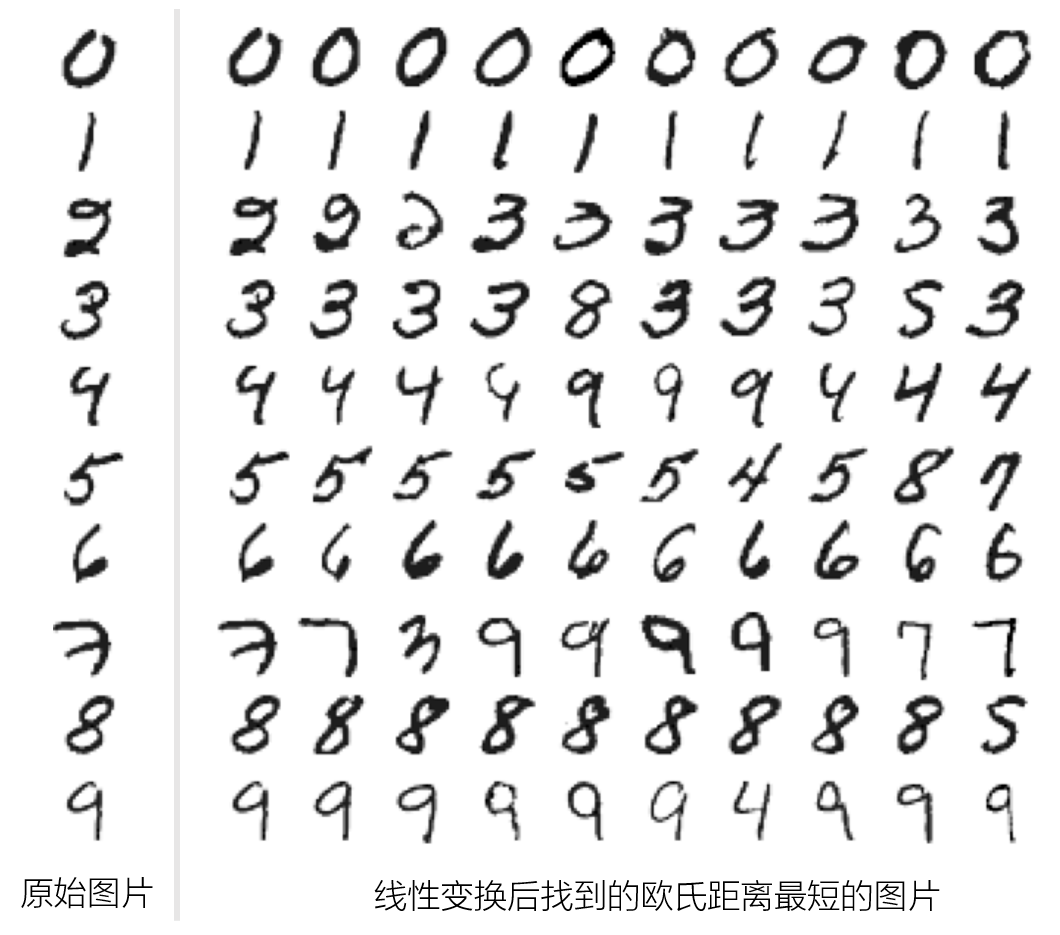
\includegraphics[width=0.66\linewidth]{Z_Resources/ss-perm_mnist-knn}
    \caption{通过对比低维投影得到的最相似样本}
    \label{fig:ss-perm:mnist-knn}
\end{figure}
%
可以看出,低维的投影相似的图片,其原始图片也十分相似。
%
因此,攻击者可以通过分析隐层表征,得到特征拥有方的数据分布、数据之间的关系,乃至数据分布随着时间变化的变化等信息。
%
以疫情防控期间的口罩检测为例,假设某公司A采用了某公司B的“口罩检测”模型来判断员工是否按照规定佩戴了口罩,并采用拆分学习(或其他需要发送隐层表征给公司B的方式)在公司内部监控摄像头的控制中心进行了模型部署。
%
公司B可以仅仅通过分析隐层表征,而无需其他任何复杂的攻击操作,来判断公司A的员工出现情况。
若某一天公司A传输的隐层表征与之前的隐层表征的相似度降低,则可以判断公司A出现了较大的人事变动情况。
%
这显然对公司A的隐私信息造成了严重泄露。


\textbf{隐层表征的重用攻击}:
在纵向联邦学习开始前,各参与方需要进行样本对齐操作,即按照统一的样本ID对各参与方数据库中的样本进行统一,保证在训练中各方采用的是相同的样本。
%
因此,在纵向联邦学习过程中,某一个恶意的参与方也可以将样本的隐层表征信息记录下来,并对这些进行滥用。
%
比如某电商公司A为了训练更好的推荐系统,与某社交平台B达成协议,让社交平台B提供一部分用户数据并且以纵向联邦的方式进行训练。
两者采用用户的手机号作为ID进行样本对齐。
%
在训练过程中,A公司可以存储隐层表征信息。
%
训练完成后,A公司可以将这些隐层表征信息,连同对应的手机号售卖给其他公司。
%
虽然这些隐层表征信息主要是通过B公司的数据以及底部模型产生的,但是在拆分学习的场景下,B公司缺少有效的技术手段检测或防止A公司对其滥用的行为。
%
因此,这种隐层表征的重复利用攻击也对拆分学习的安全性带来了不利影响。

综上所述,使用拆分学习或是其他暴露中间结果的隐私保护机器学习方法,必然要面对中间结果的隐私泄漏问题以及中间结果可能被再次利用的问题。


\subsection{问题定义}
本文考虑如下的隐私保护机器学习问题。
两方$P_0, P_1$分别持有部分数据$X$和模型参数$\Theta$,并且要进行模型的推断或训练,具体如下:
\begin{enumerate}[label=(\arabic*)]
    \item 模型推断:计算 $Y = f(X; \Theta)$,其中$f$表示模型的推断函数,是公开的。要求在推断过程中,模型参数$\Theta$和各方数据$X$,以及其他中间结果尽可能不暴露。
    模型预测值$Y$只暴露给设定的结果获取方,可能是$P_0$或$P_1$,也可以是其他方。
    \item 模型训练:计算 $\Theta' = g(X; \Theta)$,其中$g$表示模型的训练函数,其输出为更新后的参数。
    比如对于梯度下降法,$g(X;\Theta) = \Theta - \alpha \partial L(X;\Theta) / \partial \Theta$,其中$L$表示损失函数,$\alpha$是学习率。
    要求在训练过程中,模型参数$\Theta, \Theta'$,各方数据$X$,以及其他中间结果尽可能不暴露。
\end{enumerate}

在上述的隐私保护机器学习过程中,我们新增一个第三方$P_2$,其自身不带任何模型参数或数据,仅为$P_0$和$P_1$的计算提供辅助作用。
此外,我们假设各个参与方在执行特定的算法(协议)时,会遵守协议进行计算,但是可能地利用其在执行协议中接收到的信息来获取其他参与方的隐私数据。
同时,任何参与方之间不会通过共谋(Collusion)来获取其他参与方的数据。
%
这个设定在密码学中被称为半可信安全性(Semi-Honest Security)设定或诚实但好奇(Honest-but-Curious)设定,在许多隐私保护机器学习算法的设计中被采用~\cite{wagh2019securenn,mohassel2018aby3,riazi_2018_chameleon}。
\section{方法描述}
本节我们描述实现隐私保护神经网络运算的方法,包括了线性计算和非线性计算两个部分。
%
我们用$\langle \cdot \rangle$表示秘密分享状态下的数值,$\langle x \rangle_i$ 表示 $P_i$所拥有的$x$的分享值,$\pi$表示排列函数。
%
我们用$UV = W$表示秘密分享采用的Beaver三元组,用于计算$XY = Z$。
%

\subsection{基于秘密分享的线性运算}
由于本章的设定是两方拥有数据和模型,外加第三方辅助计算,因此本章采用两方加法分享(Additive Sharing)作为秘密分享方案。
%
秘密分享一般在有限域上进行,在本章中我们将其定义在整数环$\mathbb Z_N$上。
%
$\mathbb Z_N$表示模$N$的整数环,其元素为$\{0, 1, \cdots, N - 1\}$。
所有的计算都通过模$N$进行,也就是将自然数运算的结果对$N$取余数。
%
在$\mathbb  Z_N$上两方加法分享的基本运算如下:
\begin{itemize}
    \item $\mathsf{Share}(x)$:
    将一个数$x \in \mathbb Z_N$分享给$P_0$和$P_1$。
    具体而言,分享方(可以是$P_0, P_1$或其他外部参与方)产生随机数$r \stackrel{\$}{\gets} \mathbb Z_N$($\stackrel{\$}{\gets}$表示等概率地从集合中选取),然后将$\langle x \rangle_0 := r$发送给$P_0$,将$\langle x \rangle_1 := x - r$发送给 $P_1$。
    我们用$\langle  x \rangle$表示$x$处于分享状态。

    \item $\mathsf{Reconst}(\langle x \rangle, P_i)$:
    将分享状态的$\langle x \rangle$恢复给$P_i$方(默认$P_i$为$P_0,P_1$双方)。
    $P_0$和$P_1$分别把$\langle x \rangle_0, \langle x \rangle_1$发送给$P_i$,然后$P_i$计算$x = \langle x \rangle_0 + \langle x \rangle_1$。

    \item $\mathsf{Add}(\langle x \rangle, y)$:
    将一个分享状态的数$\langle x \rangle$与一个公开的数$y$相加。
    将其和记为$\langle z \rangle$,$P_0$本地计算$\langle z \rangle_0 = \langle x \rangle_0 + y$,$P_1$本地计算$\langle z \rangle_1 = \langle x \rangle_1$。
    
    \item $\mathsf{Add}(\langle x \rangle, \langle x \rangle)$:
    将两个分享状态的数$\langle x \rangle, \langle y \rangle$相加。
    将其和记为$\langle z \rangle$,$P_{i\in \{0, 1\}}$本地计算$\langle z\rangle_i = \langle x \rangle_i + \langle y \rangle_i$。
    
    \item $\mathsf{Mul}(\langle x \rangle, y)$:
    将一个分享状态的数$\langle x \rangle$与一个公开的数$y$相乘。
    将其乘积记为$\langle z \rangle$,$P_{i\in \{0, 1\}}$本地计算$\langle z\rangle_i = \langle x \rangle_i y$。

    \item $\mathsf{Mul}(\langle x \rangle, \langle y \rangle)$:
    将两个分享状态的数$\langle x \rangle, \langle y \rangle$相乘。
    该过程较为复杂,需要借助Beaver三元组才可以进行。
    本章使用辅助第三方$P_2$来产生Beaver三元组。
    %
    具体步骤如下:
    \begin{enumerate}
        \item $P_2$产生$u, v\stackrel{\$}{\gets} \mathbb Z_N$,并计算$w = uv$。
        
        \item $P_2$执行$\mathsf{Share}(u), \mathsf{Share}(v), \mathsf{Share}(w)$,将$u, v, w$分享给$P_0, P_1$。
        
        \item $P_0$和$P_1$执行$\mathsf{Reconst}(\langle x \rangle - \langle u \rangle), \mathsf{Reconst}(\langle y \rangle - \langle v \rangle)$。

        \item $P_0$计算$\langle  z \rangle_0 = (x - u)(y - v) + (x - u)\langle v \rangle_0 + \langle u \rangle_0 (y - v) + \langle w \rangle_0$;$P_1$计算$\langle  z \rangle_1 = (x - u)\langle v \rangle_1 + \langle u \rangle_1 (y - v) + \langle w \rangle_1$。
    \end{enumerate}
    我们可以简单地验证 $z = xy$。
\end{itemize}

可以看到,秘密分享的所有运算中,仅有两个分享状态的数的乘法需要参与方之间进行信息传输。
%
且对于任何一个参与方$P_i$,如果其没有关于$x$的信息,则$x - u$对其来说是一个均匀分布的随机变量;同理,如果没有关于$y$的信息,则$y - v$ 对其来说也是一个均匀分布的随机变量。
%
因此,使用上述方法计算两个分享状态的数的乘法并不会暴露任何隐私信息。
%
事实上,上述秘密分享的运算均满足信息论安全性(Information-Theoretic Security),也就是在各个参与方不共谋的情况下,即使攻击者拥有无穷的计算力,他依然无法获得任何原始数据的信息\cite{beaver1992efficient}。

尽管上述的秘密分享运算只定义在单独一个整数上,很容易可以看出我们也可以将其定义到任何向量、矩阵,乃至张量(Tensor)的运算上,乘法也可以拓展为矩阵乘法、张量乘法等一切满足乘法分配律的运算,且安全性得到完全保留。

\subsubsection{定点数编码}
一般的神经网络的计算都定义在实数上,并且以浮点数的格式进行实际的计算。
%
但是上述的秘密分享运算只适用于整数。
%
因此,我们需要定义实数与浮点数点相互转换机制。
%
我们把整数环$\mathbb Z_N$分为两个部分:$[0, \lfloor N/2 \rfloor)$ 用于表示正数,而$[\lfloor N/2 \rfloor, N)$用于表示负数。
%
对于一个实数$x$,我们首先计算其正整数部分$\lfloor x\cdot P \rceil$,其中$P$表示放缩系数(Scaling Factor),用于控制小数部分的精度。
%
然后对于负数,我们则用$N - 1$对其进行相减,得到 $N - \lfloor x\cdot P \rceil$。
%
综上所述,将实数编码为整数的函数为:
\begin{equation}
    x_Z := \mathsf{Encode}(x) = x \cdot P \bmod N.
\end{equation}
%
相应的解码函数为:
\begin{equation}
    x := \mathsf{Decode}(x_Z) = \begin{cases}
        x_Z / P         & \text{如果 $x < N/2$ ($x$是正数)}, \\
        (N - x_Z) / P     & \text{否则 ($x$ 是负数)}.
    \end{cases}
\end{equation}
%
同时,为了保证编码和解码的准确性,实数$x$必须处于区间$\big[ -\dfrac{N}{2P}, \dfrac{N}{2P} \big)$中。


\subsubsection{乘法截断}
当两个被编码的实数$x_Z, y_Z$进行乘法后,其乘积的放缩系数也是各自放缩系数的乘积:
\begin{equation}
    x_Zy_Z = (xP \bmod N)(yP \bmod N) = xyP^2 \bmod N = [(xy)_F \bmod N \cdot P] \bmod N.
\end{equation}
%
若乘法执行了$L$次,则对应的放缩系数会变为$P^L$,此时乘积是$xyP^L$,很可能已经超出了$[-N/2, N/2)$这一个有效的解码范围,导致解码错误。
%
为此,我们需要在每次乘法之后进行截断操作,即
\begin{equation}
    z = xy \Rightarrow z_Z = \Big\lfloor \dfrac{(x_Z y_Z) \bmod P}{P} \Big\rceil.
\end{equation}
%

在明文状态下,该截断操作可以直接执行。
%
对于秘密分享状态下的正整数,则截断操作会更为复杂。
%
SecureML~\cite{mohassel2017secureml}论文的作者采用了两方直接本地截断(Local Truncation)的办法,也就是:
\begin{equation}
    \langle z_Z \rangle_i \gets \langle x_Zy_Z \rangle_i / P.
\end{equation}
%
注意这里的除法需要考虑符号位。
此处我们直接用“/”来表示整数除法($\lfloor \cdot / \cdot \rceil$)。
%
可以证明,该方法能够以很大的概率产生和在明文上截断最多相差1的结果。

\begin{theorem}[本地截断]
\label{thm:ss-perm:local-truncation}
    对于在$\mathbb Z_N$下分享状态的数$\langle x \rangle_0, \langle x \rangle_1$,且$|x| \le x_\text{max} < N/2$,则最多有
    $\dfrac{2x_\text{max}}{N}$的概率使得$\langle x \rangle_0/P + \langle x \rangle_1/P\notin [x/P - 1, x/P + 1]$。
\end{theorem}
\begin{proof}
    首先考虑$\langle x \rangle_0, \langle x \rangle_1$符号相反的情况,此时在$\mathbb Z$上有$\langle x \rangle_0 + \langle x \rangle_1 = x$。
    注意到因为四舍五入的误差不超过0.5,因此对于任何$a + b = c \in \mathbb R$,有$\lfloor a \rceil + \lfloor b \rceil \in [\lfloor c \rceil - 1, \lfloor c \rceil + 1]$。
    将其带入$\langle x \rangle_0/P + \langle x \rangle_1/P = x/P$,即可得到$\langle x \rangle_0, \langle x \rangle_1$符号相反时该结论成立。
    接下来考虑$\langle x \rangle_0, \langle x \rangle_1$符号相同的概率。
    %
    假设$-x_\text{max} \le x \le 0$,则需要满足 
    %
    \begin{equation}
    \begin{cases}
        0 \le \langle x \rangle_0 < N/2, \\
        0 \le x - \langle x \rangle_0 < N/2.
    \end{cases}
    \end{equation}
    第二行可以改为$N/2 < \langle x \rangle_0 - x \le N$,只有$\langle x \rangle_0 \in (N/2 + x, N/2)$时,上述条件成立。
    再考虑$-x_\text{max} \le x \le 0$,得到其概率小于 $2x_\text{max}/N$。
    对于$0 \le x \le x_\text{max}$的情况,我们也可以得到类似结果$\langle x \rangle_0 \in [N/2, N/2 + x)$,证明完毕。
\end{proof}
%
上述定理表明,采用简单的本地截断方法,其截断出错的概率也是很小的。
%
但是小概率的截断错误在神经网络训练中也是不可接受的,下面我们举例说明。
%
比如我们令$N = 2^{64}$,放缩系数$P = 2^{20}$,$|x|, |y| \le 2^{8}$,则经过一次乘法$z = xy$,$|z| \le 2^{56}$。
%
通过\autoref{thm:ss-perm:local-truncation}可以得到,此时截断出错的概率小于$2 \times 2^{56} / 2^{64} = 1/128$。
%
考虑到神经网络的计算中会涉及到较大的矩阵,则截断出错很容易在计算中出现。
%
不仅如此,我们可以看到该截断产生的误差是非常大的,可以到接近$\dfrac{N}{2P}$的量级。
%
如此巨大的误差将会给神经网络的训练或推断带来重大的影响,使得其结果毫无意义。
%
因此,我们必须采取措施避免简单的“本地截断”带来的误差。


根据\autoref{thm:ss-perm:local-truncation}的分析,可以看到截断错误是否发生与$\langle x \rangle_0$有关。
%
具体而言,当$|\langle x \rangle_0| \in (N/2-x_\text{max}, N/2]$时,才有可能产生截断错误。
%
因此,对$x$进行截断时,我们只需要让$P_0$检查$|\langle x \rangle_0|$是否在可能截断错误的范围内,再对其进行缩小处理。如果$|\langle x \rangle_0|$在该范围内,若$\langle x\rangle_0$为正数(在$[0, N/2)$区间),则$P_0$首先计算$\langle x \rangle_0 \gets \langle x \rangle_0 - N/4$,并发送“+”给$P_1$,$P_1$执行$\langle x \rangle_1 \gets \langle x \rangle_1 + N/4$。
%
注意到这种方法会暴露关于$x$的范围信息,但是其暴露的概率较小(等价于定理\autoref{thm:ss-perm:local-truncation}中截断出错的概率),且即使暴露,很大概率也只暴露一个宽度为$x_\text{max}$左右的范围。
%
考虑到神经网络的计算过程中的变量元素都很多,暴露其中很少部分元素的范围不会造成实质性的隐私泄露。
%
总而言之,本章所以出的方法是将小概率的截断错误转化为小概率的部分元素范围泄露。
因为在神经网络的训练和推断中往往涉及到数量庞大的大规模的矩阵运算,即使是小概率的截断错误,由于其错误的误差极大,也会导致神经网络的训练崩溃或输出无意义结果。
而相比之下,泄露少量元素的范围并不会让攻击者窃取有意义的隐私数据。
%
因此,本章提出的截断方法更适合神经网络的安全计算。

\subsubsection{优化的秘密分享乘法}
为了进一步提高效率,我们注意到上述截断过程可以与秘密分享的乘法过程绑定,从而实现减少通信量的目的。
%
在秘密分享的乘法中,$P_0$和$P_1$之间要进行两次通信来重构$x - u$和$y - v$,分别是$P_0$发送自身对应的分享值和$P_1$发送自身对应的分享值。
%
假设$P_1$先发送自身的秘密分享值,则$P_0$收到分享值后,可以先计算乘积分享值$\langle z \rangle_0$,同时利用该值检查是否有需要进行缩小,再把是否需要缩小的信息连同$\langle x \rangle_0 - \langle u \rangle_0, \langle y \rangle_0 - \langle v \rangle_0$一同发给$P_1$。
%
这样不会在秘密分析乘法中带来任何额外的通信。
%
我们将优化后的秘密分享张量乘法定义在\autoref{alg:ss-perm:ss-mul}中。


\begin{algorithm}[h!]
\caption{秘密分享乘法$\mathsf{SSMul}$}
\label{alg:ss-perm:ss-mul}
    \begin{algorithmic}[1]
    \Require{秘密分享的张量$\langle X \rangle, \langle Y \rangle$;乘法函数$f_\text{mul}$;放缩系数$P$;结果范围$z_\text{max}$}
    \Ensure{秘密分享的张量$\langle Z = \dfrac{XY}P \rangle$}
    \State 各方将默认乘法设置为$f_\text{mul}$ \LineComment{视具体情况,可以是逐元素乘法、矩阵乘法等}
    \State $P_2$生成Beaver三元组$UV=W$($U, V$形状和$X, Y$相同,其元素从$\mathbb Z_N$中均匀采样),并将其秘密分享给$P_0, P_1$
    \State $P_1$发送$\langle X \rangle_1 - \langle U \rangle_1, \langle Y \rangle_1 - \langle V \rangle_1$给$P_0$
    %
    \State $P_0$恢复出
    $X - U = \langle X \rangle_0 - \langle U \rangle_0 + \langle X \rangle_1 - \langle U \rangle_1, 
     Y - V = \langle Y \rangle_0 - \langle V \rangle_0 + \langle Y \rangle_1 - \langle V \rangle_1$
    %
     \State $P_0$计算出$\langle Z \rangle_0 = (X - U)(Y - V) + (X - U)\langle V \rangle_0 + \langle U \rangle_0 (Y - V) + \langle W \rangle_0$
    %
    \State $P_0$找出$\langle Z \rangle_0$中满足 $\langle Z \rangle_0[i] \in (N/2 - z_\text{max}, N/2)$的下标$i$集合,记作$I_\text{large}$;同理找到$\langle Z \rangle_0[i] \in [-N/2, -N/2 + z_\text{max})$的下标$i$集合,记作$I_\text{small}$
    %
    \NewlineComment{此处下标为把张量$\langle Z \rangle_0$转化为1维向量的下标}
    %
    \For{$i \in I_\text{large}$}
        \State $P_0$ 更新 $\langle Z \rangle_0[i] \gets \langle Z \rangle_0[i] - N/4$
    \EndFor
    \For{$i \in I_\text{small}$}
        \State $P_0$ 更新 $\langle Z \rangle_0[i] \gets \langle Z \rangle_0[i] + N/4$
    \EndFor
    %
    \State $P_0$发送$\langle X \rangle_0 - \langle U \rangle_0, \langle Y \rangle_0 - \langle V \rangle_0, I_\text{small}, I_\text{large}$给$P_1$
    %
    \State $P_1$恢复出$X - U, Y - V$
    \State $P_1$计算出$\langle Z \rangle_1 = (X - U)\langle V \rangle_1 + \langle U \rangle_1(Y - V) + \langle W \rangle_1$
    %
    \For{$i \in I_\text{large}$}
        \State $P_1$ 更新 $\langle Z \rangle_1[i] \gets \langle Z \rangle_1[i] + N/4$
    \EndFor
    \For{$i \in I_\text{small}$}
        \State $P_1$ 更新 $\langle Z \rangle_1[i] \gets \langle Z \rangle_1[i] - N/4$
    \EndFor
    \end{algorithmic}
\end{algorithm}




\subsection{基于随机排列的激活函数计算}
神经网络中除了矩阵的线性运算(加法、乘法),另一种不可或缺的运算是非线性激活函数(Activation Function)。
%
若没有激活函数,则整个神经网络将退化为一个线性映射。
%
由于激活函数是非线性的,甚至无法使用多项式表示,因此其对密码学方案不友好,当前许多研究采用混淆电路或其他精心设计的MPC协议计算,产生了大量的开销,同时由于其中采用了近似计算,可能还会带来神经网络的精确度损失~\cite{mohassel2017secureml,liujian2017minionn,mishra2020delphi}。
%
另一方面,如果将神经网络中间结果发送给第三方来算激活函数,则第三方可以根据中间结果来反推神经网络的权重。
%
为此,本章提出利用随机排列来安全地解决激活函数的计算。


对$n$个元素进行随机排列(Random Permutation),表示将$n$个元素打乱顺序,总共有$n!$种不同的排列顺序。
%
注意到,排列的数目随着$n$的增长呈现出超指数(Super-Exponential)增长,因此即使是较少的元素,其可能的排列顺序也是天文数字。
%
比如,仅仅10个元素有360多万种排列($\approx 2^{22}$);而当元素个数增长到100,则可能的排列数超出$2^{524}$。
%
如此大量的排列个数,使得从随机排列中猜测出原排列的概率几乎为0。
%
考虑到神经网络中间结果往往是包含大量元素的张量,我们可以认为对其进行随机排列后几乎可以消除所有原始张量的信息。
%
并且注意到,神经网络的激活函数是作用于每个元素上的(Element-Wise),因此打乱顺序后执行激活函数与执行激活函数后再打乱顺序是等价的。

因此,我们可以让$P_0$和$P_1$对秘密分享的神经网络中间结果执行随机排列后,再恢复到$P_2$上。
%
$P_2$随即在随机排列后的明文上计算出激活函数的值,再将其重新分享给$P_0$和$P_1$两方。
%
$P_0$和$P_1$可以通过逆向排列,恢复出最终结果的分享值。
%
注意到,在此过程中,$P_0$和$P_1$必须采用同样的随机排列,否则会导致恢复错误。
%
此外,我们还可以通过(在元素数量不足够大时)添加扰动元素;对Tanh、Sigmoid等对称激活函数在随机排列中加入随机翻转来进一步提高安全性。
上述方法实现简单,本文不再赘述。
%
我们将该方法在\autoref{alg:ss-perm:perm-act}中进行具体描述。


\begin{algorithm}[h!]
    \caption{基于随机排列的激活函数计算方法$\mathsf{PermNonlinear}$}
    \label{alg:ss-perm:perm-act}
        \begin{algorithmic}[1]
        \Require{秘密分享的张量$\langle X \rangle$;激活函数$f$}
        \Ensure{秘密分享的张量$\langle Y = f(X) \rangle$}
        %
        \State $P_0$ 生成一个随机排列 $\pi \stackrel{\$}{\gets} \text{Perm}(\text{Size}(X))$
        \LineComment{Size$(X)$表示张量$X$的元素个数}
        \State $P_0$ 将$\pi$ 发送给$P_1$
        %
        \State $P_0, P_1$分别将$\pi[\langle X \rangle_0], \pi[\langle X \rangle_1]$发送给$P_2$
        %
        \State $P_2$恢复出$\pi[X] = \pi[\langle X \rangle_0] + \pi[\langle X \rangle_1]$,并计算出$\pi[f(X)] = f(\pi[X])$
        \State $P_2$将$\pi[f(X)]$分享给$P_0, P_1$
        \State $P_0$和$P_1$分别计算得到$\langle Y \rangle_0 = \pi^{-1} \langle \pi[f(X)] \rangle_0, \langle Y \rangle_1 = \pi^{-1} \langle \pi[f(X)] \rangle_1$
    \end{algorithmic}
\end{algorithm}


通过该方法,我们可以极大的降低激活函数的计算开销。我们在\autoref{tab:ss-perm:relu}中对本方法和对比算法的ReLU激活函数计算的通信轮次/通信量进行对比。
%
表中的$p$是一个质数(一般为三位数),$k$是混淆电路的安全性参数(Security Paramter),一般大于128。
%
注意到,本方法的开销已经考虑了下一节所用基于关联随机性(Correlated Randomness)的通信优化算法。

\begin{table}[t]
    \caption{不同算法ReLU开销对比}
    \label{tab:ss-perm:relu}
    \centering
    \begin{tabular}{ccc}
    \toprule
    算法 & 通信轮次 & 通信量(比特) \\ 
    \midrule
    本方法 & $3$ & $3L$ \\
    SecureNN\cite{wagh2019securenn} & $11$ & $8L\log_2 p + 32L + 2$ \\
    ABY3\cite{mohassel2018aby3} & $6 + \log L$ & $105L$ \\
    混淆电路\cite{rouhani2018deepsecure} & $4$ & $k(3L - 1)$ \\
    \bottomrule
    \end{tabular}
\end{table}

\subsection{基于关联随机性的通信优化}
两方具有关联随机性,可以理解为两方有一个同样的伪随机数生成器(Pseudo-Random Generator),可以使得其每次采样时产生同样的随机数。
%
通过关联随机性,我们可以进一步降低上述的秘密分享乘法(\autoref{alg:ss-perm:ss-mul})以及基于随机排列的激活函数计算方法(\autoref{alg:ss-perm:perm-act})的通信复杂度~\cite{riazi_2018_chameleon}。
%

\textbf{优化\textsf{SSMul}}:具体而言,$P_0$和$P_2$分享一个伪随机数生成器$G_\text{beaver}$。
在\autoref{alg:ss-perm:ss-mul}第2行中,$P_2$使用$G_\text{beaver}$产生Beaver三元组给$P_0$的分享:$\langle U \rangle_0, \langle V \rangle_0, \langle W \rangle_0 \gets G_\text{beaver}$。
同时,$P_0$自身也可以产生这些分享,因此$P_2$无需再将这些分享值发送给$P_0$。


\textbf{优化\textsf{PermNonlinear}}:$P_0$和$P_1$分享一个伪随机数生成器$G_\text{perm}$,用于在\autoref{alg:ss-perm:perm-act}中产生同样的随机排列。因此,\autoref{alg:ss-perm:perm-act}第2行可以改为$P_1$通过$G_\text{perm}$产生随机排列,从而减少一次通信。
%
此外,$P_0$和$P_2$分享一个伪随机数生成器$G_\text{share}$,用于$P_2$产生$\langle \pi[f(X)] \rangle_0$时。此时在\autoref{alg:ss-perm:perm-act}第5行时,$P_2$无需再将$\langle \pi[f(X)] \rangle_0$发送给$P_0$,从而减少一次通信。


\subsection{隐私保护神经网络框架实现}
基于上述的秘密分享乘法和基于随机排列的激活函数,我们已经能够实现基本的全连接神经网络的推断和训练。
%
在神经网络中有如下的操作:
\begin{itemize}
    \item 线性运算:加法、减法、乘法(包含矩阵乘法和逐元素相乘);
    \item 激活函数运算:比如ReLU、Sigmoid、Tanh等;
    \item 本地计算:包括了矩阵转置(Transpose)等。
\end{itemize}
%
对于加法和乘法,我们采用秘密分享以及本章提出的\autoref{alg:ss-perm:ss-mul}来实现。
对于减法$x - y$,我们将其转换为$x + (-y)$,而负数在秘密分享中也只需要双方本地将该数取负号(在$\mathbb Z_N$中,$-x = N - x$)。
%
对于激活函数,采用上述的\autoref{alg:ss-perm:perm-act}实现。
%
综上,我们将全连接神经网络的推断和训练在\autoref{alg:ss-perm:train}和\autoref{alg:ss-perm:infer}中进行描述。
%
\begin{algorithm}[h!]
    \caption{隐私保护神经网络推断$\mathsf{PriavteNNInfer}$}
    \label{alg:ss-perm:train}
        \begin{algorithmic}[1]
        \Require{秘密分享的输入$\langle X \rangle$;秘密分享的第$i$层权重$\langle W \rangle_i$;偏置$\langle \bvec b \rangle_i$;激活函数$f_i$}
        \Ensure{秘密分享的神经网络输出$\langle Y\rangle$}
        %
        \State $\langle H \rangle_0 \gets \langle X \rangle$
        \For{$i = 0$ to $L -1$} \LineComment{$L$为总层数}
            \State $\langle Z_{i + 1} \rangle = \mathsf{SSMul}(\langle H_i \rangle, \langle W_i \rangle^T, \text{矩阵乘}) + \langle \bvec b_i \rangle$
            \State $\langle H_{i + 1} \rangle = \mathsf{PermNonlinear}(\langle Z \rangle_{i+1}, f_i)$
        \EndFor
        \State \Return $\langle H_L\rangle$
    \end{algorithmic}
\end{algorithm}

%
\begin{algorithm}[h!]
\caption{隐私保护神经网络训练$\mathsf{PriavteNNTrainStep}$}
\label{alg:ss-perm:infer}
    \begin{algorithmic}[1]
    \Require{秘密分享的输入特征$\langle X \rangle$ 和标签$\langle Y \rangle$;秘密分享的第$i$层权重$\langle W \rangle_i$;偏置$\langle \bvec b \rangle_i$;激活函数$f_i$;学习率$\alpha$}
    \Ensure{一次梯度下降后更新的权重和偏置}
    %
    \State 各方执行$\langle Y' \rangle \gets \mathsf{PrivateNNInfer}(\langle X \rangle, (\langle W \rangle_i, \langle \bvec{b} \rangle_i, f_i))$,
        并且在执行过程中保留中间变量$\langle Z_1 \rangle, \cdots, \langle Z_L \rangle$和$\langle H_1 \rangle, \cdots, \langle H_L \rangle$
    %
    \State $\langle G_L \rangle \gets 2 \cdot (\langle Y \rangle - \langle Y' \rangle)$
    %
    \For{$i = L - 1$ to $0$} \LineComment{$L$为总层数}
        \State $\langle G'_{i + 1} \rangle \gets \mathsf{PermNonlinear}(\langle Z_{i+1} \rangle, \dfrac{df_i}{dx})$ \LineComment{$\dfrac{df_i}{dx}$也是逐元素函数}
        \State $\langle G_{i + 1} \rangle \gets \mathsf{SSMul}(\langle G'_{i+1} \rangle, \langle G_{i+1} \rangle, \text{元素乘})$
        \State $\langle G_{i} \rangle \gets \mathsf{SSMul}(\langle G_{i+1} \rangle, \langle W_i \rangle, \text{矩阵乘})$ \LineComment{对权重进行了转置}
        \State $\langle \bvec b_i \rangle \gets \langle \bvec b_i \rangle - \alpha \cdot \mathsf{sum}(\langle G_i \rangle, \mathsf{axis}=0)$ \LineComment{\textsf{sum}可以表示为秘密分享的加法}
        \State $\langle W_i \rangle \gets \langle W_i \rangle - \alpha \cdot \mathsf{SSMul}(\langle G_i \rangle^T, \langle H_i \rangle, \text{矩阵乘})$
    \EndFor
\end{algorithmic}
\end{algorithm}

%
\section{安全性分析}
本章提出的隐私保护神经网络的线性计算部分采用秘密分享进行设计,在半可信安全性设定下满足信息论安全~\cite{demmler2015aby}。
%
因此,本节讨论基于随机排列的非线性激活函数计算的安全性。
%
尽管前文已经展示了可能的随机排列个数随着元素个数$n$的增长而超指数增长,本节采用了更加精确的量化手段基于分析。
%
具体而言,本节采用了距离相关性(Distance Correlation)作为安全性指标,对于随机排列以及简单的线性变换(拆分学习中直接暴露中间结果的情况)进行了分析,显示了随机排列带来的隐私泄露极小。

\subsection{距离相关性}
距离相关性(Distance Correlation)~\cite{szekely2007dcor,szekely2009brownian_dcor}是一种统计学上的相关性度量,可以度量任意两个高维向量之间的相关性。
相对于常用的皮尔逊相关性系数(Pearson Correlation Coefficient),距离相关性可以对任意两个不同维度的高维随机向量进行建模,并且可以捕获非线性的相关性,只有在两个随机向量完全无关时才会为0。
%
因此,距离相关性适合用来分析高维向量之间的关联性。

\begin{definition}[距离相关性]
    对于两个随机向量$X \in \mathbb R^p, Y\in \mathbb R^q$,距离相关性的定义为
    \begin{equation}
        \textnormal{DCOR}(X, Y) = \dfrac{\mathcal{V}(X, Y)^2}{\sqrt{\mathcal{V}(X, X)^2\mathcal{V}(Y, Y)^2}},
    \end{equation}
    其中$\mathcal{V}$表示距离协方差(Distance Covariance),定义如下
    \begin{equation}
        \mathcal{V}(X, Y)^2 = \dfrac{1}{c_pc_q} \int_{\mathbb R^{p + q}}
        \dfrac{|f_{X, Y}(t, s) - f_X(t)f_Y(s)|^2}{\Vert c_p \Vert^{p+1}\Vert c_q \Vert^{q+1}}dtds,
    \end{equation}
    其中,$c_p, c_q$为两个常数,$\Vert \cdot \Vert$表示欧几里得范数(Euclidean Norm)。
\end{definition}

除去上述的定义为,距离协方差还可以通过
\begin{equation}
\begin{split}
    \mathcal{V}(X, Y)^2 = 
    & \quad \mathbb E \Vert X-X'\Vert \Vert Y -Y'\Vert +\mathbb E\Vert X -X' \Vert \mathbb E \Vert Y -Y' \Vert
    \\ & 
    - \mathbb E\Vert X-X'\Vert  \Vert Y -Y''\Vert - \mathbb E \Vert X -X''\Vert  \Vert Y -Y' \Vert
\end{split}
\end{equation}
来计算,其中$(X, Y), (X', Y'), (X'', Y'')$是相互独立的。
%
通过上式可以以采样的方式来估算距离相关性。

\subsection{随机线性变换的距离相关性}
现在我们研究随机线性变换后的向量与随机变换之前的向量的距离相关性。
我们用$\angle[\cdot, \cdot]$表示两个向量之间的夹角。
\begin{theorem}
\label{thm:ss-perm:linear-dcov}
    令$X\in \mathbb R^n$是一个随机的$n$维随机向量,令$Y = AX$,
    %
    其中 $A \in \mathbb R^{n \times d}$是一个随机线性变换,并且满足在单位正交变换下概率不变,即$P(A) = P(AT)$, $T$是$n$维单位正交矩阵(Orthonormal Matrix)。
    %
    则
    \begin{equation}
    \label{eq:ss-perm:linear-dcov1}
            \mathop{\mathbb E}_A \mathcal{V}(X, AX)^2 = a\mathcal{V}(X, X)^2,
    \end{equation}
    以及    
    \begin{equation}
    \label{eq:ss-perm:linear-dcov2}
        \mathop{\mathbb E}_A \mathcal{V}(AX, AX)^2 = {a^2S_1 + b^2S_2 - 2S_3'},
    \end{equation}
    其中 $S_1 = \mathbb \Vert X - X'\Vert^2, S_2 = \left( \mathbb E \Vert X - X'\Vert \right)^2, S_3 = \mathbb E \Vert X - X' \Vert \Vert X - X'' \Vert$,\\
    $S' = \mathbb E \left[ g(\angle [X - X', X - X'']) \cdot \Vert X - X'\Vert \Vert X - X'' \Vert \right]$,
    以及
    $g_A(\theta) = \mathbb E_A \dfrac{\Vert A\bvec x \Vert \Vert A\bvec y \Vert}{\Vert \bvec x \Vert \Vert \bvec y \Vert} $,
    $a = \mathbb E_A \dfrac{\Vert A\bvec x \Vert}{\Vert \bvec x \Vert}$,
    $b = \sqrt{\mathbb E_A \dfrac{\Vert A\bvec x \Vert^2}{\Vert \bvec x \Vert^2}}$,$\bvec x, \bvec y$为任意的$n$维向量,且夹角为$\theta$。
\end{theorem}
\begin{proof}
我们用$\mathbb E$来简略表示$\mathbb E_{X,X',X''}$。
%
首先注意到$\mathbb E_A\mathbb E\Vert X - X' \Vert \Vert A(X - X') \Vert = \mathbb E \left[ \Vert X - X'\Vert^2 \mathbb E_A \dfrac{\Vert A(X - X') \Vert }{\Vert X - X'\Vert} \right]$。
%
可以看出$\mathbb E_A \dfrac{\Vert A(X - X') \Vert }{\Vert X - X'\Vert}$和$X$无关,因此可以进一步写成
$\mathbb E \Vert X - X'\Vert^2 \cdot \mathbb E_A \left[ \dfrac{\Vert A(X - X') \Vert }{\Vert X - X'\Vert} \right] = a\mathbb E \Vert X - X'\Vert^2$。
%
同理可得\autoref{eq:ss-perm:linear-dcov1}的推导。
另外
\begin{equation}
\begin{split}
    \mathbb E_A \mathbb E{\Vert AX - AX' \Vert \Vert AX - AX'' \Vert} = 
    \mathbb E \mathbb E_A \Vert A(X - X') \Vert \Vert A(X - X'') \Vert \\
    =
    \mathbb E \left[ \Vert X - X' \Vert \Vert X - X'' \Vert \mathbb E_A \dfrac{\Vert A(X - X') \Vert \Vert A(X - X'') \Vert}{\Vert X - X' \Vert \Vert X - X'' \Vert}  \right].
\end{split}
\end{equation}

下面我们证明$\mathbb E_A \dfrac{\Vert A\bvec x\Vert \Vert A \bvec y\Vert }{\Vert \bvec x \Vert \Vert \bvec y \Vert}$只和$\bvec x, \bvec y$之间的夹角有关。
%
由于对$\bvec x, \bvec y$放缩不影响结果,我们考虑两对$n$维向量$\bvec x, \bvec y$与$\bvec x', \bvec y'$满足$\Vert \bvec x \Vert = \Vert \bvec x' \Vert = \Vert \bvec y \Vert = \Vert \bvec y' \Vert = 1$,
且$\bvec x, \bvec y$和$\bvec x', \bvec y'$的夹角均为$\theta$。
%
令$\bvec e_1 = \bvec x/\Vert x \Vert, \bvec e_2 = (\bvec y - \bvec y \cdot \bvec x/\Vert \bvec x \Vert) / \Vert \bvec y - \bvec y \cdot \bvec x/\Vert \bvec x \Vert \Vert$,
且$\bvec e_3, \cdots, \bvec e_n$是与$\bvec e_1, \bvec e_2$正交的任意$n-2$组单位正交向量组。
%
此时,有$\bvec x = \bvec e_1, \bvec y = \cos \theta \bvec e_1 + \sin \theta \bvec e_2$。
%
同理,我们也可以把$\bvec x'$和$\bvec y'$表示为$\bvec e_1'$与$\cos \theta \bvec e'_1 + \sin \theta \bvec e'_2$。
%
此时$(\bvec e_1, \cdots, \bvec e_n)$与$(\bvec e'_1, \cdots, \bvec e'_n)$是$\mathbb R^n$的两组单位正交基,因此存在单位正交矩阵$T$使得$T\bvec e_i = \bvec e'_i$。
%
也就是$\dfrac{\Vert A\bvec x \Vert\Vert A\bvec y \Vert}{\Vert \bvec x\Vert \Vert \bvec y \Vert} = \dfrac{\Vert AT\bvec x' \Vert\Vert AT\bvec y' \Vert}{\Vert \bvec x'\Vert \Vert \bvec y' \Vert}$。
%
注意到$P(A)=P(AT)$,因此$\mathbb E_A f(A) = \mathbb E_A f(AT)$,令$f(A) = \dfrac{\Vert A\bvec x \Vert\Vert A\bvec y \Vert}{\Vert \bvec x\Vert \Vert \bvec y \Vert}$ 可以得到$f(A)$仅仅和$\theta$有关。
%
于是有$\mathbb E_A \mathcal{V}(AX, AX) = b^2 S_1 + a^2 S_2 - 2S_3'$,也就是\autoref{eq:ss-perm:linear-dcov2}。
\end{proof}

\autoref{thm:ss-perm:linear-dcov}显示出,当$A$是一个具有旋转不变性(Rotation Invariance)分布的随机线性变换时,$\mathcal{V}(X, AX)/\mathcal{V}(X, X)$的期望值只和$A$有关,而和$X$的具体分布无关。
%
同时,$\mathbb E_A \mathcal{V}(AX, AX)$随着$g_A(\theta)$的提升而降低。
%
我们可以进一步证明,$g_A(\theta)$在$[0, \pi/2]$上是单调递减的。
%
\begin{proposition}
    $g_A(\theta)$在$[0, \pi/2]$上是单调递减的。
\end{proposition}
%
\begin{proof}
    由于$A$的分布具有旋转不变性,不妨令
    $\bvec x = \begin{bmatrix}
        \cos \theta/2 \\ \sin \theta/2 \\ \bvec 0   
    \end{bmatrix}$
    和
    $\bvec y = \begin{bmatrix}
        \cos \theta/2 \\ \sin \theta/2 \\ \bvec 0
    \end{bmatrix}$,
    此时有 $g_A(\theta) = \mathbb E_A \Vert A\bvec x\Vert \Vert A \bvec y\Vert$。
    我们可以对$A$在前两个维度构成的平面上进行旋转角度$\alpha$:
    \begin{equation}
        AT = A \begin{bmatrix}
            \cos \alpha & \sin \alpha & O \\
            -\sin \alpha &\cos \alpha & O \\
            O & O & E
        \end{bmatrix}.
    \end{equation}
    此时有:
    \begin{equation}
    \begin{split}
        \mathbb E_A \Vert A\bvec x \Vert \Vert A \bvec y \Vert = \mathbb E_A \Vert AT \bvec x \Vert \Vert AT \bvec y \Vert = \mathbb E_A \mathbb E_T \Vert AT \bvec x \Vert \Vert AT \bvec y \Vert \\
        = \mathbb E_A \mathbb E_\alpha 
        \left[
        \Vert \cos(\alpha - \theta/2)\bvec a_0 - \sin (\alpha - \theta/2) \bvec a_1\Vert 
        \cdot
        \Vert \cos(\alpha + \theta/2)\bvec a_0 - \sin (\alpha + \theta/2) \bvec a_1\Vert
        \right],
    \end{split}   
    \end{equation}
    其中,$\bvec a_0, \bvec a_1$是$A$的前两列。
    %
    对$\theta$进行求导,得到:
    \begin{equation}
        \begin{split}
            & \dfrac{d\mathbb E_\alpha \Vert A\bvec x \Vert \Vert A\bvec y \Vert}{d\theta} = 
            -(\Vert \bvec a_0 \Vert^2 + \Vert \bvec a_1 \Vert^2)\sin \theta \cdot \\
            & \int_{\alpha=0}^{2\pi} 
                \text{Sign}[(\Vert \bvec a_0 \Vert^2 - \Vert\bvec a_1\Vert^2)\cos 2 \alpha] - 
                (\bvec a_0 \cdot \bvec a_1) \sin 2\alpha + 
                (\Vert \bvec a_0 \Vert^2 + \Vert\bvec a_1\Vert^2) \cos \theta d\alpha.
        \end{split}
    \end{equation}
    注意到积分号中的前两项积分后为0,整个式子为负数,因此我们可以得出$g(\theta)$在$[0, \pi/2]$中单调递减。
\end{proof}

直观角度理解,$S'$项反应了分布$X$的“集中度”对距离方差带来的影响。
%
当$X$中的各个点分布在很接近的方向上时,$\angle[X - X', X - X'']$变小,因此$S'$变大,从而导致$\mathcal{V}(AX, AX)$变小,随之$\text{DCOR}(X, AX)$变大。
%
也就是说,$X$的分布的方向越集中,则与其随机线性投影的距离相关性有更大可能变大。
%
在极端情况下,$X$分布在一条线上,则$S' = S_3$取得最大值。
%
同时,变换$A$若能尽可能保留数据点之间的距离,则也能提高变换前后的距离相关性。
%
如果$A$是保距变换(Distance-Preserving Transformation),则显然$\text{DCOR}(X, AX) = 1$。


%
在神经网络中,我们一般采用$\mathcal N(0, \sigma^2)$来初始化全连接权重。
%
考虑$W \sim \mathcal N(0, \sigma^2)^{n \times d}$,此时考虑对向量$\bvec e_1$计算$\mathbb E_A \Vert W\bvec e_1 \Vert$与$\sqrt{\mathbb E_A \left[\Vert W\bvec e_1 \Vert^2 \right]}$,对应卡方分布(Chi-Square Distribution)的均值以及其平方根的均值。
%
因此可以得到
$a = \mathbb E \sqrt{w_1^2 + \cdots + w_d^2} = \sigma \sqrt{2} \Gamma(d + 1/2) / \Gamma(d) \approx \sigma \sqrt{d - 1/2}$(对于较大的 $d$),
$b = \mathbb E \left[ {w_1^2 + \cdots + w_d^2} \right] = \sigma\sqrt{d}$。
%
再考虑$\bvec x = \bvec e_1, \bvec y = \cos \theta \bvec e_1 + \sin \theta \bvec e_2$,可以得到
\begin{equation}
    g_A(\theta) = \mathbb E_A \Vert A\bvec x \Vert \Vert A \bvec y \Vert = \int_{\bvec x, \bvec y \in \mathbb R^d} e^{-\dfrac{\Vert \bvec x \Vert^2 + \Vert \bvec y \Vert^2}{2\sigma^2}}
\Vert \bvec x \Vert \Vert \cos \theta \bvec x + \sin \theta \bvec y \Vert d\bvec x d\bvec y.
\end{equation}

通过数值模拟,我们也注意到:
\begin{equation}
\label{eq:ss-perm:linear-dcor-estimation}
\begin{split}
    \mathop{\mathbb E}_A \text{DCOR}(X, AX) & = \mathop{\mathbb E}_A \dfrac{\mathcal{V}(X, AX)^2}{\mathcal{V}(X, X)\mathcal{V}(AX, AX)}
    \\
    &\approx \dfrac{\mathbb E_A \mathcal{V}(X, AX)^2}{\mathcal{V}(X, X) \mathbb E_A \mathcal{V}(AX, AX)}
    \\
    &= \sqrt{\dfrac{a^2(S_1 + S_2 - 2S_3)}{a^2S_1 + b^2S_2 - 2S_3'}}.
\end{split}
\end{equation}
%
也就是我们可以用距离协方差的均值来估算距离相关性的均值(尽管一般情况下$\mathbb E X/Y \ne \mathbb E X/\mathbb E Y$),这给我们提供了新的估算距离相关性的手段。
%


\subsection{随机排列的距离相关性分析}
我们首先注意到,对于$\bvec x \in \mathbb R^d$和随机排列$\pi$,可以得到如下特性:
\begin{itemize}
    \item $\mathbb E_\pi \pi[\bvec x] = [\mathbb E\bvec x, \cdots, \mathbb E\bvec x] = M(\bvec x)$,其中我们定义$\mathbb E\bvec x = 1/d \cdot \sum_{i=1}^d x_i$。
    \item 对于任意排列$\pi'$,有$(\pi'[\bvec x] - \mathbb E_{\pi}\pi[\bvec x])^T \bvec 1 = 0$。
    \item 对于任意排列$\pi'$,有$\Vert \pi'[\bvec x] - M(\bvec x)\Vert = \Vert \bvec x - M(\bvec x)\Vert$。
\end{itemize}
%
通过以上特性可以归纳出,随机排列后的向量分布在以$M(\bvec x)$为中心,$\Vert \bvec x - \mathbb E_\pi \pi[\bvec x]\Vert$为半径的一个$d - 2$维超球面(Hypersphere)上,且该超球面所在的子空间为$\{\bvec x: \bvec x \in \mathbb R^d, \bvec 1^T\bvec x = 0\}$。
%
我们将$\pi[\bvec x] - M(\bvec x)$记为$r(\pi[\bvec x])$(误差向量),并考察其在子空间$\bvec 1^T \bvec y = 0$上面的投影。
%

\begin{theorem}
\label{thm:ss-perm:perm-dist}
    对于任何一个在子空间$\bvec 1^T \bvec y = 1$上的单位向量$\bvec y$,我们有:
    $\mathbb E_\pi \left[r(\pi[\bvec x])  \cdot \bvec y\right] = 0$,以及$\textnormal{Var}_\pi \left[ r(\pi[\bvec x])\cdot \bvec y \right] = \dfrac{1}{n - 1} \Vert r(\bvec x) \Vert^2$。
\end{theorem}
%
\begin{proof}
首先,$\mathbb E_\pi  \left[r(\pi[\bvec x]) \cdot \bvec y\right] = \sum_{i}^n \mathbb E_\pi [x_{\pi[i]} - \mathbb E\bvec x] y_i = \sum_{i=1}^d 0 \cdot \bvec y = 0$。然后考虑方差,
我们有:
\begin{equation}
\begin{split}
    \text{Var}\left[ r(\pi[\bvec x])\cdot \bvec y \right] = \mathbb E_\pi \left[\sum_{i,j=1}^n  r(\pi[\bvec x])_i y_i r(\pi[\bvec x])_j y_j \right].
\end{split}
\end{equation}
我们分为$i = j$和$i \ne j$两种情况进行讨论。
\begin{itemize}
    \item $i = j$:
    \begin{equation}
        \mathbb E_\pi \sum_{i = 1}^d r(\pi[\bvec x])_i^2 y_i^2 = \sum_{i=1}^d \mathbb E_\pi \left[ \Vert r(\pi[x])_i\Vert^2 \right] y_i^2 = \sum_{i=1}^d \dfrac{1}{d} \Vert r(\bvec x) \Vert^2 y_i^2 = \dfrac{\Vert r(\bvec x)\Vert^2}d.
    \end{equation}
    
    \item $i \ne j$:此时我们注意到$\sum_{i=1}^d r(\pi[\bvec x])_i = 0$和$\sum_{i=1}^d y_i = 0$两个等式,代入可得:
    \begin{equation}
    \label{eq:ss-perm:dcor-perm0}
        \mathbb E_\pi \sum_{i=1}^d  \sum_{j = 1, j\ne i}^d r(\pi[\bvec x])_i r(\pi[\bvec x])_j y_i y_j = \sum_{i=1}^d  \sum_{j = 1, j\ne i}^d \mathbb E_\pi \left[ r(\pi[\bvec x])_i r(\pi[\bvec x])_j \right] y_i y_j.
    \end{equation}
    %
    注意到,对于任意$i, i'$,$\pi[i] = i'$ 都是等概率的,因此,我们可以进一步得到:
    \begin{equation}
    \begin{split}
        \mathbb E_\pi \left[ r(\pi[\bvec x])_i r(\pi[\bvec x])_j \right] = \dfrac{1}{d(d-1)}\sum_{\substack{i',j'=1\\i'\ne j'}}^d r(\bvec x)_{i'} r(\bvec y)_{j'} \\
        = \dfrac{1}{d(d-1)}\sum_{i'=1}^d -r(\bvec x)_{i'}^2  = -\dfrac{1}{d(d-1)}\Vert r(\bvec x) \Vert^2.
    \end{split}
    \end{equation}
    代入\autoref{eq:ss-perm:dcor-perm0}中,得到
    \begin{equation}
        -\dfrac{\Vert r(\bvec x) \Vert^2 }{d(d-1)}\sum_{i=1}^d  \sum_{j = 1, j\ne i}^d y_i y_j = -\dfrac{\Vert r(\bvec x) \Vert^2 }{d(d-1)}\sum_{i=1}^d -y_i^2 = \dfrac{\Vert r(\bvec x) \Vert^2 }{d(d-1)}.
    \end{equation}
\end{itemize}
将上述两项相加,可以得到$\textnormal{Var}_\pi \left[ r(\pi[\bvec x])\cdot \bvec y \right] = \dfrac{1}{n - 1} \Vert r(\bvec x) \Vert^2$。
\end{proof}

\autoref{thm:ss-perm:perm-dist}表明,随机排列的误差向量几乎均匀地分布在超球面上,因为其没有对任何一个方向有偏好性(在任何一个方向上的投影的均值和标准差都是一样的)。
%
我们现在考虑随机投影$Y = AX, A \sim \mathcal N(0, 1)^{n\times d}$。
由于$A$中的元素符合正态分布,因此我们可以得到:$\Vert M(Y) \Vert^2 \approx  \dfrac{1}{n} \Vert Y \Vert^2$和$\Vert r(\pi[Y]) \Vert \approx \Vert Y \Vert$(因为$\pi[Y] = M(Y) + r(\pi[Y])$)。
%
这种情况下,$\pi[Y]$的误差向量的幅度显著高于其均值向量的维度。
%
由于误差向量的分布没有方向上的偏好性,我们可以假设$\mathcal{V}[X, r(Y)] = 0$以及$\mathcal{V}(M(Y), r(Y)) = 0$。
%
其次,由于误差向量的幅度远大于均值向量,我们可以假设
\begin{equation}
\mathcal{V}[\pi[Y], \pi[Y]] = \mathcal{V}[M(Y) + r(Y), M(Y) + r(Y)] > \mathcal{V}[M(Y), M(Y)].
\end{equation}
%
综合上述两点假设以及距离协方差的性质,我们可以得到:
\begin{equation}
\begin{split}
    \text{DCOR}(X, \pi[Y]) &= \mathcal{V}(X, \pi[Y]) / (\mathcal{V}[X, X] \mathcal{V}[\pi[Y], \pi[Y]]) \\
    & < \mathcal{V}(X, M(Y)) / (\mathcal{V}[X, X] \mathcal{V}[M(Y), M(Y)]) \\
    & = \text{DCOR}(X, M(Y)).
\end{split}
\end{equation}
注意到$M(Y)$是$X$的一维随机投影,可以进一步得到:
\begin{equation}
    \mathbb E_A \text{DCOR}(X, \pi[AX]) < \mathbb E_A \text{DCOR}(X, M(AX)) = \mathbb E_{B \sim \mathcal N(0, 1)^{n\times 1}} \text{DCOR}(X, BX).
\end{equation}
%
上述推导表明,$X$和$\pi[AX]$之间的距离相关性要小于$X$与其一维投影之间的距离相关性。
也就是说,从距离相关性的角度,随机投影再加上随机排列后泄漏的信息小于一维投影泄漏的信息。
%
这说明本章提出的基于随机排列的非线性激活函数计算基本可以认为是安全的。


\subsection{数值模拟}
为了验证上述对于距离相关性的分析以及呈现随机排列与随机投影对距离相关性的影响,本节我们进行了数值模拟实验来测算不同分布的数据经过随机投影/随机排列后的距离相关性。
%

我们令数据的原始维度均为100维,并且符合如下分布:
\begin{itemize}
    \item \textbf{正态分布}:数据从$\mathcal N(0, 1)^{100}$中抽取
    (注:我们用$\mathcal D^{n}$表示长度为$n$的随机向量,其中每个元素的分布都为$\mathcal D$且相互独立)。
    \item \textbf{均匀分布}:数据从$\mathcal U(0, 1)^{100}$中抽取。
    \item \textbf{稀疏分布}:数据中每个点有0.1的概率为1,否则则为0。
    \item \textbf{子空间分布}:数据分布在一个20维的子空间附近。
    具体而言,数据表示为$X = AH + E$,其中$H \sim \mathcal N(0, 1)^{20}, A \sim \mathcal N(0, 1/{20^2})^{20\times 100}, E \sim \mathcal N(0, 0.1)^{100}$。
\end{itemize}


\begin{figure}[h!]
    \centering
    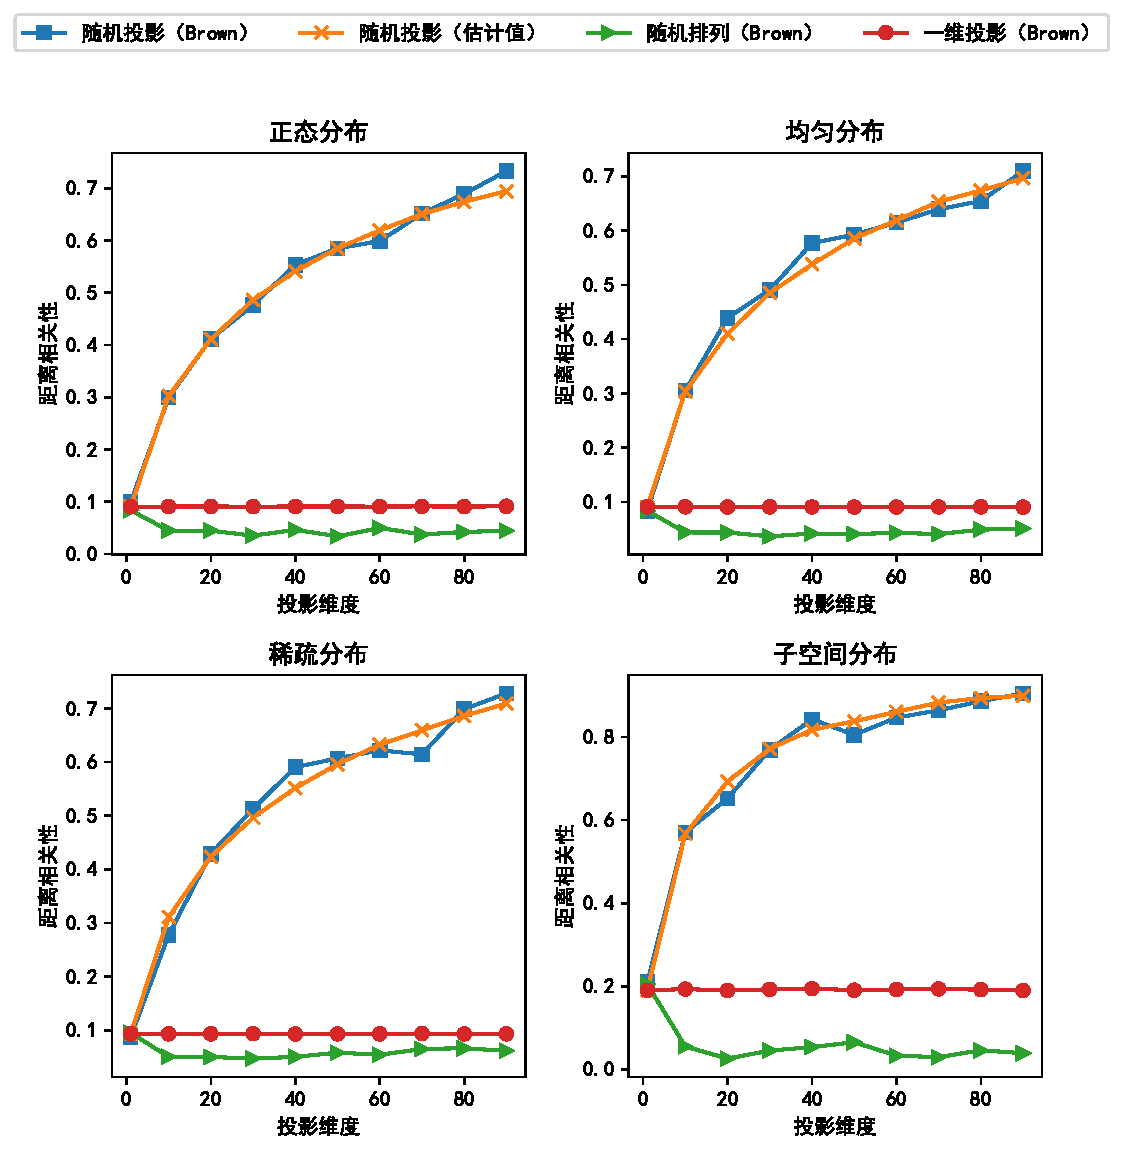
\includegraphics[width=\linewidth]{Z_Resources/ss-perm_dcor-estimation}
    \caption{各种数据分布下随机投影和随机排列的距离相关性}
    \label{fig:ss-perm:dcor-estimation}
\end{figure}


对于每个分布,我们采样1万个点(记作$X$),然后使用高斯分布的矩阵投影得到$Y = WX$,最后对投影后的向量进行随机排列得到$\pi[Y]$。
%
我们采用文献~\cite{szekely2009brownian_dcor}中的基于布朗运动(Brownian Motion)的方法对距离相关性进行数值计算(标记为“Brown”),同时也使用\autoref{eq:ss-perm:linear-dcor-estimation}对随机投影的距离相关性进行估算(标记为“估计值”),并一同呈现在\autoref{fig:ss-perm:dcor-estimation}中。
%


上述数值模拟表明,随机投影后的数据与原始数据具有较大的距离相关性,且投影后的维度越高,距离相关性越大。
%
而本文在投影后的数据上进一步采用随机排列,极大减少了距离相关性。
且无论投影维度变化,其距离相关性一直小于一维投影的距离相关性,验证了本节的理论分析结论。
\section{实验分析}
为了验证本章所提出的隐私保护神经网络框架的实用性,本节对本章的算法进行了实现。
%
我们基于Python的Numpy计算库~\cite{stefan_2011_numpy}实现了秘密分享的计算,其中秘密分享的整数环被选为$\mathbb Z_{2^{64}}$,因为64位整数能被计算机原生支持,可以方便地使用各种编程语言操作。
%
我们选择放缩系数为$2^{23}$,也就是对于任何实数(浮点数$x$),其整数表示为$x \cdot 2^{23}$。
此时定点数计算的精度达到$2^{-23}$,与32位浮点数的精确位一致~\cite{ieee_754_float},因此在该精度下神经网络的计算几乎不会有精度损失。
%
对于秘密分享中的通信交互,我们采用Python原生的套接字(Socket)接口进行编程,通过在节点之间建立持久化TCP连接的方式来交互数据,仅需初始化时的三次握手建立连接,防止其他上层协议带来的通信延迟。
同时我们采用流的方式进行数据读写,使用Pickle对变量进行打包。
%

\subsection{实验设置}
本节的实验在一台装备了16核Intel CPU,64GB内存的服务器上进行。
我们通过Linux自带的tc(Traffic Control)内核命令在本地网络(Localhost)上模拟了广域网(WAN, Wide Area Network)的带宽和延迟。
%
我们将WAN的带宽设置为80Mbps,将往返时间(Round Trip Time)设置为40ms。
%
这样的设置符合普通的家用宽带标准。
%
在实验开始之前,我们将训练数据以及初始化的神经网络权重秘密分享在$P_0$和$P_1$上。
%
我们对比了两个较新的密码学隐私保护神经网络方案,分别是SecureNN~\cite{wagh2019securenn}和ABY3~\cite{mohassel2018aby3}。
%
由于上述框架原始论文的开源代码未提供或无法运行,我们使用LatticeX-Rosetta库~\cite{latticex_rosetta}的SecureNN框架,以及TF-Encrypted库~\cite{tf_encrypted}的ABY3框架。
%
我们令所有的实验至少重复运行了10次,并把实验结果取平均值。


\begin{table}[h!]
\caption{逻辑回归的运行时间和通信量}
\label{tab:ss-perm:logistic}
\renewcommand{\arraystretch}{0.8}
\begin{tabular}{@{}cccrrrrrr@{}}
    \toprule
    \multicolumn{1}{l}{}     & \multicolumn{1}{l}{}    &    & \multicolumn{3}{c}{运行时间(秒)}       & \multicolumn{3}{c}{通信量(Mb)}       \\ 
    \cmidrule(lr){4-6}\cmidrule(lr){7-9}
    \multicolumn{1}{l}{输入维度} & \multicolumn{1}{l}{批大小} &    & 本方法            & SecureNN & ABY3  & 本方法            & SecureNN & ABY3  \\ 
    \cmidrule(lr){1-3}\cmidrule(lr){4-6}\cmidrule(lr){7-9}
    \multirow{4}{*}{100}     & \multirow{2}{*}{64}     & 推断 & \textbf{0.099} & 0.219    & 0.500 & \textbf{0.103} & 0.226    & 0.372 \\ \cmidrule(l){3-3}\cmidrule(lr){4-6}\cmidrule(lr){7-9}
        &                      & 训练 & \textbf{0.279} & 0.348 & 0.534 & \textbf{0.209} & 0.391 & 0.385          \\ \cmidrule(l){2-3}\cmidrule(lr){4-6}\cmidrule(lr){7-9}
        & \multirow{2}{*}{128} & 推断 & \textbf{0.108} & 0.228 & 0.500 & \textbf{0.202} & 0.448 & 0.624          \\ \cmidrule(l){3-3}\cmidrule(lr){4-6}\cmidrule(lr){7-9}
        &                      & 训练 & \textbf{0.281} & 0.367 & 0.539 & \textbf{0.413} & 0.775 & 0.639          \\ \midrule
    \multirow{4}{*}{1000}    & \multirow{2}{*}{64}     & 推断 & \textbf{0.132} & 0.358    & 0.511 & \textbf{0.996} & 1.072    & 1.369 \\ \cmidrule(l){3-3}\cmidrule(lr){4-6}\cmidrule(lr){7-9}
        &                      & 训练 & \textbf{0.294} & 0.698 & 0.831 & 1.988          & 2.581 & \textbf{1.678} \\ \cmidrule(l){2-3}\cmidrule(lr){4-6}\cmidrule(lr){7-9}
        & \multirow{2}{*}{128} & 推断 & \textbf{0.114} & 0.558 & 0.513 & 1.975          & 2.134 & \textbf{1.884} \\ \cmidrule(l){3-3}\cmidrule(lr){4-6}\cmidrule(lr){7-9}
        &                      & 训练 & \textbf{0.334} & 1.202 & 0.837 & 3.949          & 5.121 & \textbf{3.225} \\ \bottomrule
\end{tabular}
\end{table}

\begin{table}[h!]
\caption{神经网络的运行时间和通信量}
\label{tab:ss-perm:dnn}
\renewcommand{\arraystretch}{0.8}
\centering
\begin{tabular}{@{}cccrrrrrr@{}}
    \toprule
    \multicolumn{1}{l}{}  & \multicolumn{1}{l}{} &    & \multicolumn{2}{l}{运行时间(秒)} &      & \multicolumn{2}{l}{通信量(Mb)} &       \\ \cmidrule(lr){4-6}\cmidrule(lr){7-9}
    \multicolumn{1}{l}{模型} & \multicolumn{1}{l}{批大小} &    & 本方法           & SecureNN & \phantom{12}ABY3 & 本方法            & SecureNN & \phantom{12}ABY3           \\ \cmidrule(lr){1-3}\cmidrule(lr){4-6}\cmidrule(lr){7-9}
    \multirow{4}{*}{DNN1} & \multirow{2}{*}{64}  & 推断 & \textbf{0.19}     & 0.68    & 0.75 & \textbf{0.39}     & 1.98    & 1.90  \\ \cmidrule(l){3-3}\cmidrule(lr){4-6}\cmidrule(lr){7-9}
                            &                         & 训练 & \textbf{0.54} & 1.29     & 0.88 & \textbf{0.78}  & 4.05     & 2.21  \\ \cmidrule(l){2-3}\cmidrule(lr){4-6}\cmidrule(lr){7-9}
                            & \multirow{2}{*}{128}    & 推断 & \textbf{0.20} & 1.10     & 0.92 & \textbf{0.70}  & 3.89     & 3.63  \\ \cmidrule(l){3-3}\cmidrule(lr){4-6}\cmidrule(lr){7-9}
                            &                         & 训练 & \textbf{0.59} & 2.08     & 1.78 & \textbf{1.38}  & 7.90     & 4.10  \\ \midrule
    \multirow{4}{*}{DNN2} & \multirow{2}{*}{64}  & 推断 & \textbf{1.05}     & 5.67    & 1.86 & \textbf{10.69}    & 25.18   & 17.16 \\ \cmidrule(l){3-3}\cmidrule(lr){4-6}\cmidrule(lr){7-9}
                            &                         & 训练 & \textbf{1.86} & 12.11    & 3.24 & \textbf{17.97} & 55.98    & 35.20 \\ \cmidrule(l){2-3}\cmidrule(lr){4-6}\cmidrule(lr){7-9}
                            & \multirow{2}{*}{128}    & 推断 & \textbf{1.26} & 9.88     & 3.65 & \textbf{12.54} & 43.08    & 36.09 \\ \cmidrule(l){3-3}\cmidrule(lr){4-6}\cmidrule(lr){7-9}
                            &                         & 训练 & \textbf{2.58} & 20.00    & 5.14 & \textbf{24.84} & 93.19    & 47.71 \\ \bottomrule
\end{tabular}
\end{table}


\subsection{基准测试}
我们在逻辑回归模型以及全连接神经网络上对本方法和SecureNN~\cite{wagh2019securenn}、ABY3~\cite{mohassel2018aby3}框架进行了效率的评估,包含了运行时间、网络通信量的测量。

\textbf{逻辑回归}:
对于逻辑回归模型,我们把输入维度设置为100或1000,并把样本批次大小(Batch Size)设置为64或128。
实验结果汇报在\ref{tab:ss-perm:logistic}中。
可以看出,本章提出的方法相比于对比方法,训练或推断同时减少了2 -- 4倍,并且在大多数情况下也取得了更低的通信消耗。
%



\textbf{神经网络}:
我们测试了两种全连接神经网络模型,其输入维度分别为100和1000,云层大小分别为50和500。
样本批次大小也同样设置为64和128。
实验结果汇报在\ref{tab:ss-perm:dnn}中。
%
实验结果表明,相比于逻辑回归模型,本方法在神经网络上具有更高的优越性。
本方法相比于对比方法,在训练速度上有1.5 -- 5.5倍提升,同时减少了40\% -- 80\%的通信量。
这是因为神经网络的计算中有更多的非线性激活函数计算,使得本方法更多地发挥了在激活函数上的优势。
%



%
\begin{figure}[h!]
    \centering
    \begin{subfigure}[b]{0.48\linewidth}
    \centering
    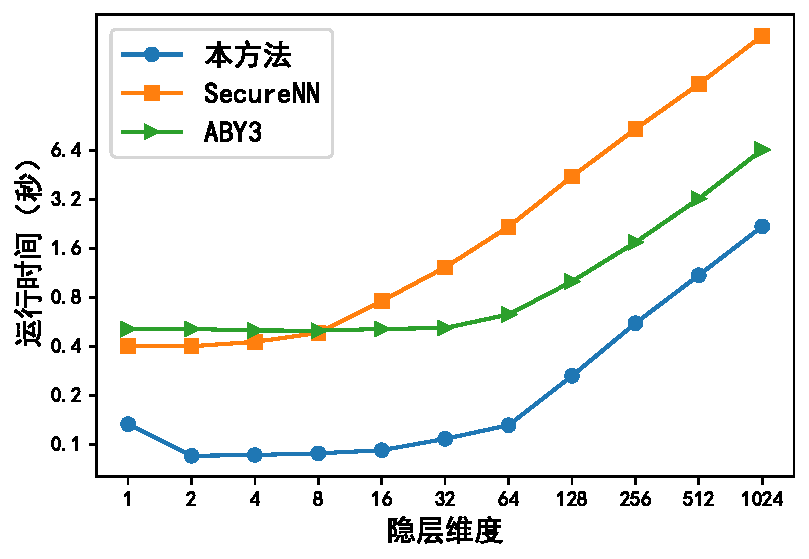
\includegraphics[width=\linewidth]{Z_Resources/ss-perm_one-layer-time.pdf}
    \caption{运行时间}
    \end{subfigure}
    %
    \begin{subfigure}[b]{0.48\linewidth}
    \centering
    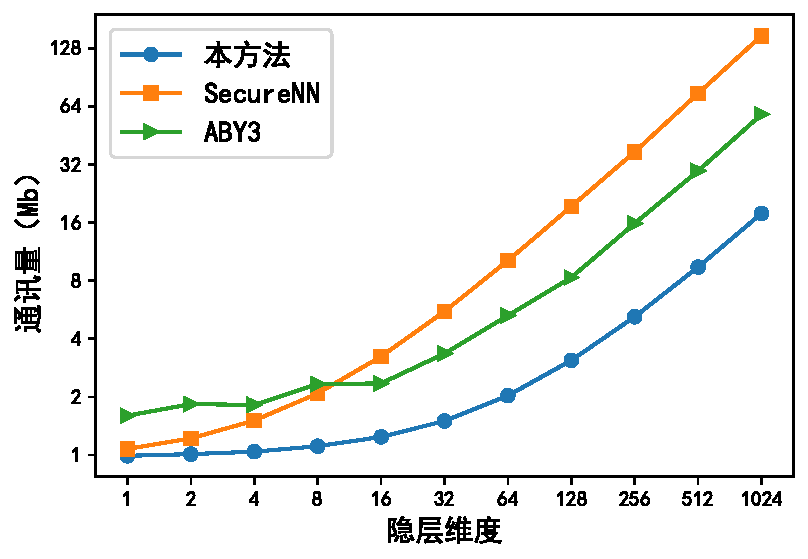
\includegraphics[width=\linewidth]{Z_Resources/ss-perm_one-layer-comm.pdf}
    \caption{总计通信量}
    \end{subfigure}
    
    \begin{subfigure}[b]{0.48\linewidth}
    \centering
    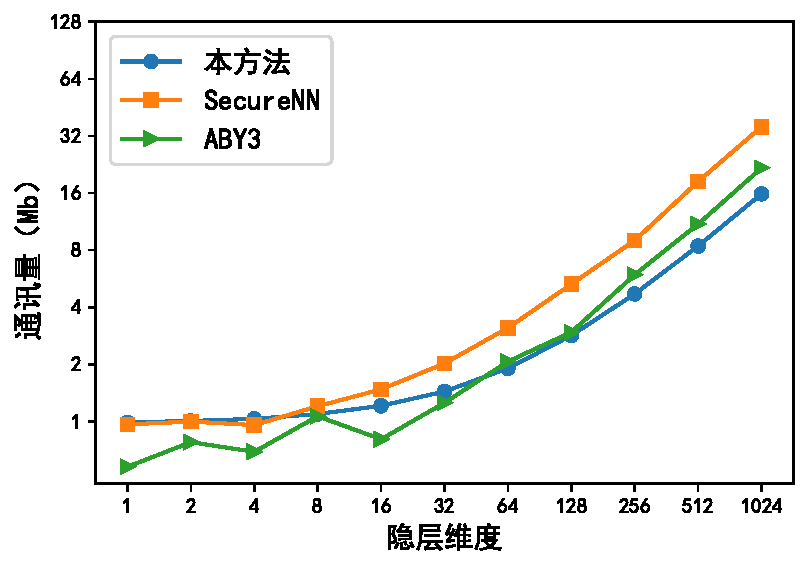
\includegraphics[width=\linewidth]{Z_Resources/ss-perm_one-layer-c01.pdf}
    \caption{$P_0$和$P_1$之间的通信量}
    \end{subfigure}
    %
    \begin{subfigure}[b]{0.48\linewidth}
    \centering
    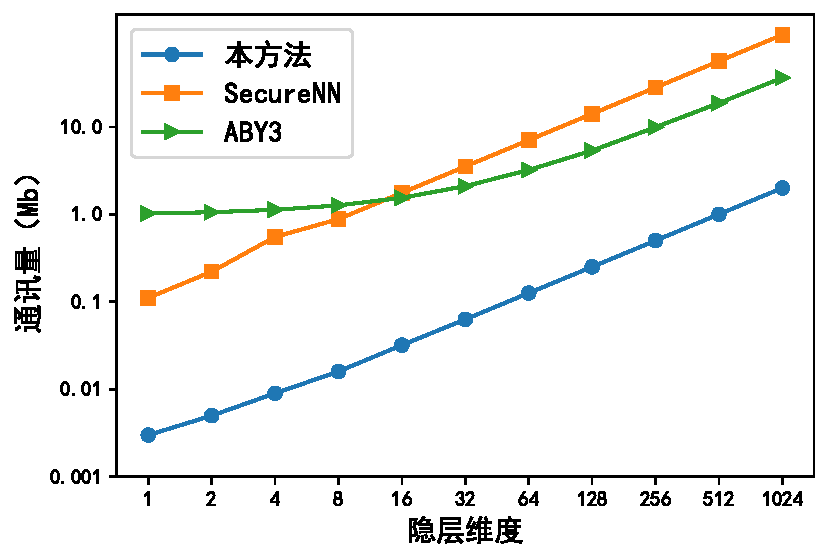
\includegraphics[width=\linewidth]{Z_Resources/ss-perm_one-layer-c2.pdf}
    \caption{$P_2$的通信量}
    \end{subfigure}
\caption{不同隐层维度时的运行时间和通信量}
\label{fig:ss-perm:layer-dim}
\end{figure}

\subsection{隐层维度对开销的影响}
为了测试本方法在不同大小的隐层上的效果,本节对本方法和对比方法在不同大小的神经网络隐层的运行时间以及通信量进行了测试,其中隐层的输入维度固定为1000。
%
本实验不仅测试了总计通信量,也测试了$P_0$和$P_1$之间的通信量和$P_2$相关的通信量。
%
实验结果呈现在\ref{fig:ss-perm:layer-dim}中。
%
可以看出,随着隐层维度逐步增加,本方法的优势逐渐扩大。
当隐层维度达到64左右时,本方法的所有通信量指标都是最低的。
%
本方法尤其减少了辅助第三方($P_2$)的通信量,相比于其他方法的通信量减少了大概1个数量级。
由于三种方法均采用秘密分享进行线性运算,因此$P_0$和$P_1$之间的通信量差距较小。

\subsection{真实数据集实验}
为了测试本章提出的方法在实际场景下的效果,本节对本章方法在真实数据下进行了实验,并且将其和明文训练进行对比,考察了训练准确率以及隐层经过随机排列后的隐私泄露程度。

\subsubsection{准确率}
为了验证本方法的训练准确率,我们在Gisette数据集~\cite{2008_gisette}和MNIST数据集~\cite{mnist}上分别使用本方法进行了训练,同时与明文对比,并绘制出验证集准确率随着训练轮数变化的曲线图在\autoref{fig:ss-perm:train}a-c中。

%
Gisette数据集~\cite{2008_gisette}是一个二分类数据集,包含了6000个训练样本和1000个测试样本,特征维度为5000。
我们用逻辑回归模型对其进行了训练。
%
MNIST数据集~\cite{mnist}是一个10分类的手写数字分类数据集,包含了60000个训练样本和10000个验证样本。
我们用两个全连接神经网络(DNN1、DNN2)对其进行训练,其结构分别为784-128-10和784-128-32-10,DNN2的第一个隐层激活函数为ReLU,其余隐层采用Sigmoid作为隐层激活函数。

实验结果表明,采用本方法的隐私保护逻辑回归和神经网络的训练曲线与明文神经网络的训练曲线几乎重合,说明本方法带来的训练精度损失可以忽略不计。

\begin{figure}[h!]
    \centering
    \begin{subfigure}[b]{0.47\linewidth}
    \centering
    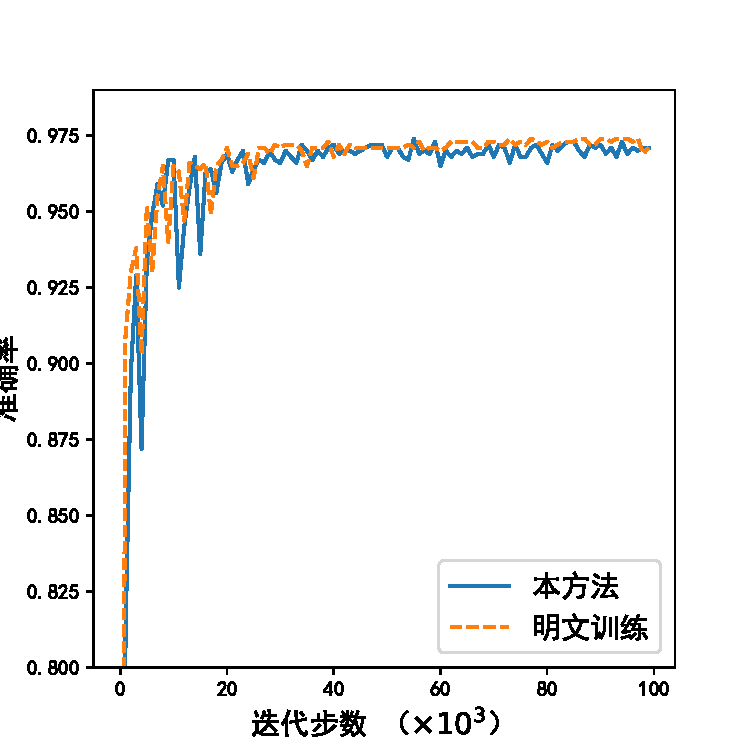
\includegraphics[width=\linewidth]{Z_Resources/ss-perm_lr.pdf}
    \caption{Gisette数据集逻辑回归训练曲线}
    \end{subfigure}
    %
    \begin{subfigure}[b]{0.47\linewidth}
    \centering
    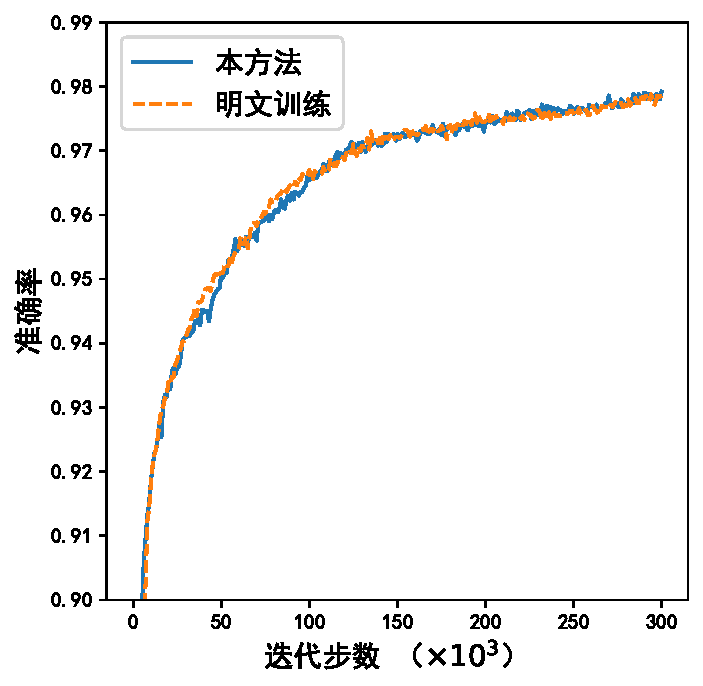
\includegraphics[width=\linewidth]{Z_Resources/ss-perm_dnn1.pdf}
    \caption{MNIST数据集DNN1训练曲线}
    \end{subfigure}
    
    \begin{subfigure}[b]{0.47\linewidth}
    \centering
    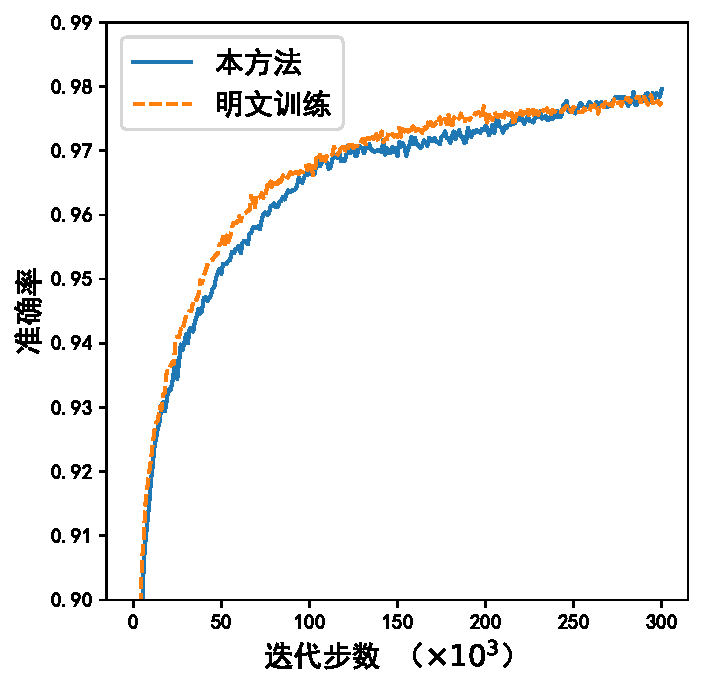
\includegraphics[width=\linewidth]{Z_Resources/ss-perm_dnn2.pdf}
    \caption{MNIST数据集DNN2训练曲线}
    \end{subfigure}
    %
    \begin{subfigure}[b]{0.47\linewidth}
    \centering
    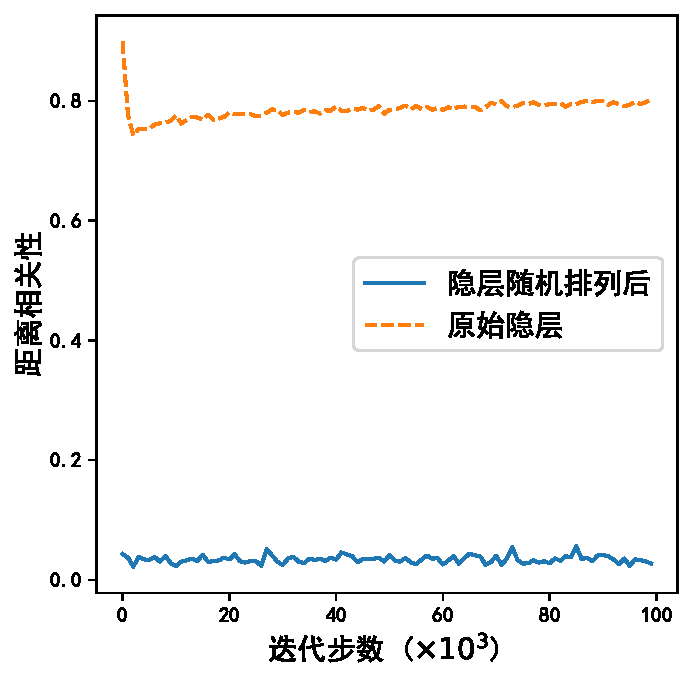
\includegraphics[width=\linewidth]{Z_Resources/ss-perm_dnn1-dcor.pdf}
    \caption{MNIST数据集DNN1隐层距离相关性}
    \end{subfigure}
\caption{在Gisette和MNIST数据集上的训练结果}
\label{fig:ss-perm:train}
\end{figure}

\subsubsection{隐层隐私泄漏情况}
我们在\autoref{fig:ss-perm:train}c中展现了DNN1隐层与输入的距离相关性,以及本方法暴露的数据(随机排列后的隐层)与输入的距离相关性。
%
可以看出,隐层与输入的距离相关性较高,在整个训练过程中维持在0.8左右的水平。
而随机排列后的隐层数据,其距离相关性大幅度降低到0.1以下,表明随机排列后的数据几乎不会带来隐私泄露。
%


另外,我们也测试了MNIST数据集中,基于隐层表征查找相似样本的结果。
%
为了考察在特殊情况下的安全性,提高隐私保护的难度,我们令一批样本全部为同一类别,因此随机排列并不能引入其他类别样本的信息。
%
实验结果呈现在\autoref{fig:ss-perm:permutation-attack}中。
%
其中最左边的列表示原始样本,蓝色方框表示框内的样本被合并为单个向量来进行随机排列。


\begin{figure}[h!]
    \centering
    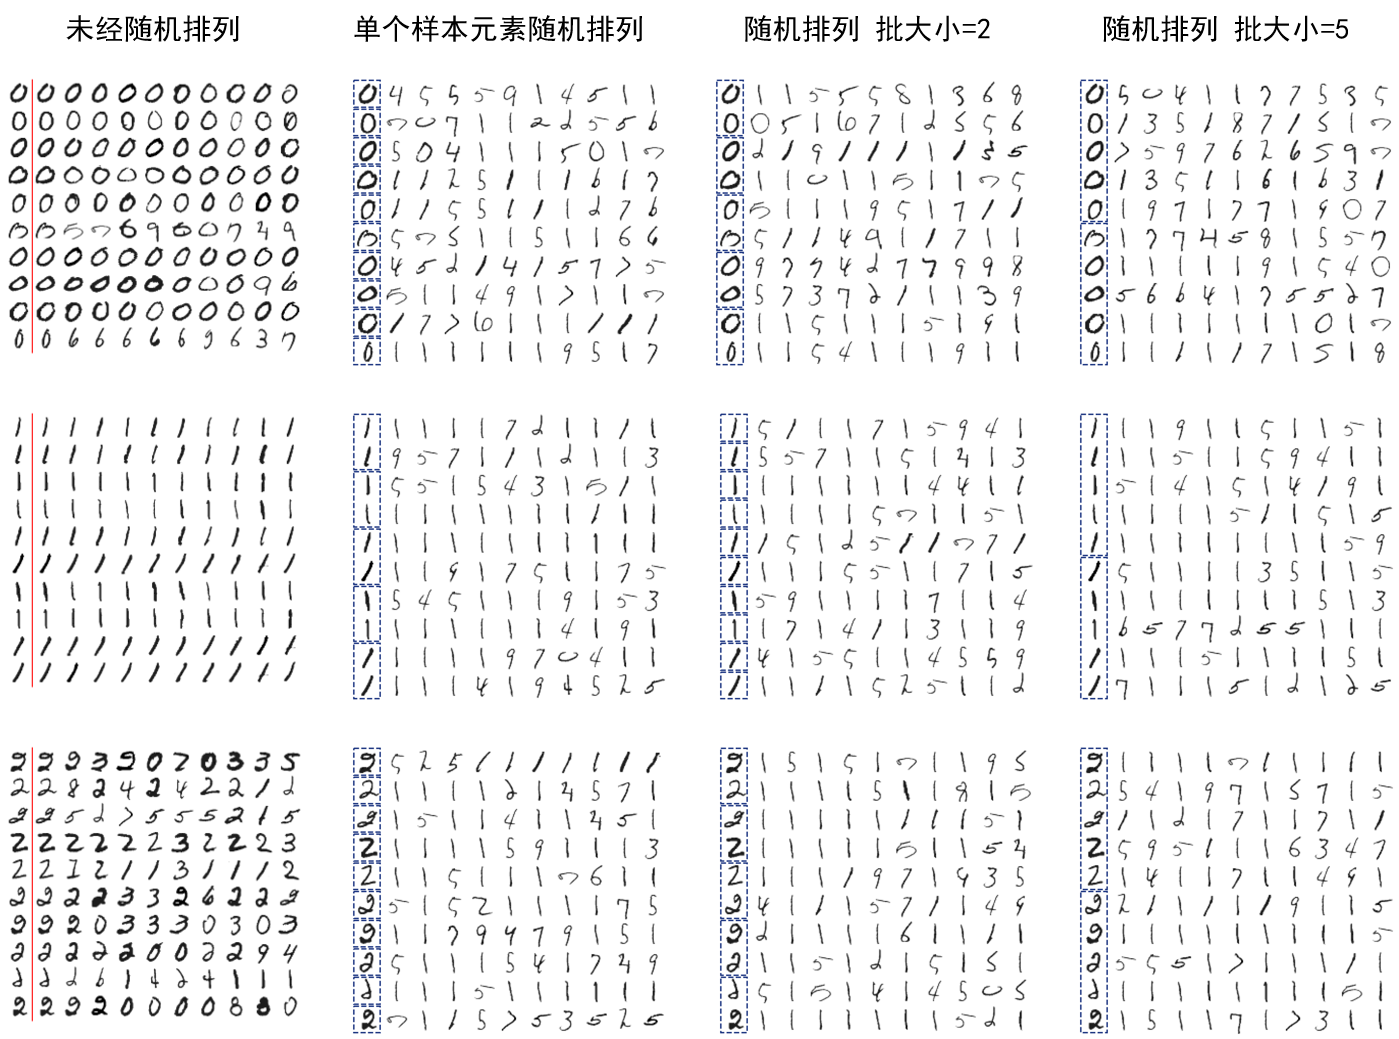
\includegraphics[width=\linewidth]{Z_Resources/ss-perm_permutation-attack.png}
    \caption{隐层表征随机排列前后的相似样本示意图}
    \label{fig:ss-perm:permutation-attack}
\end{figure}

实验结果表明,如果没有进行随机排列,也就是直接暴露隐层表征时,攻击者很容易根据隐层表征找到相似的样本。
%
而采用了随机排列之后,则攻击者找到的相似样本和原始样本无关。
%
无论原始样本属于哪个类别,找到的相似样本都是一些笔画较细的“1”等图像。
%
这是因为两个隐层表征$\bvec x, \bvec y \in \mathbb R^d$之间的距离可以用表示为
$\mathbb E_i [(x_i - y_i)^2] = \mathbb E_i [x_i^2 + y_i^2 - 2x_i y_i]$。
%
当$\bvec x, \bvec y$归一化后且$x_i, y_i$之间没有相关性时,则上式可以进一步表示为
$\mathbb E_i [x_i^2] + \mathbb E_i [y_i^2]$。
%
注意到$x_i, y_i \ge 0$。
%
因此,若$\mathbb E_i [y_i^2]$越小,就会导致$\mathbb E_i [(x_i - y_i)^2]$越小。
%
而较小的$\mathbb E_i[y_i^2]$对应是分布更加集中的$\bvec y$,其输入大概率是黑色像素较少的图片,因为MNIST数据集的图像以白色部分为主。
%

\section{本章小结}